In der Messung werden für den Frequenzbereich von 6000 bis 9000 $\si{Hz}$ Rohrlängen von $\SI{75}{mm}$ bis $\SI{600}{mm}$ vermessen.
Bei bestimmten Frequenzen bildet sich eine stehende Welle aus. Das hat Resonanz zur Folge, so dass die Schallwelle eine höhere Intensität hat.
In den folgenden 2 Abbildungen wird die Intensität gegen die Wellenlänge aufgetragen.
In der Abbildung \ref{fig.1} sind die Messwerte für die Rohrlängen : $\SI{75}{mm}, \SI{150}{mm}, \SI{225}{mm}, \SI{300}{mm}$ abbgebildet.
\begin{figure}[h!]
  \centering
  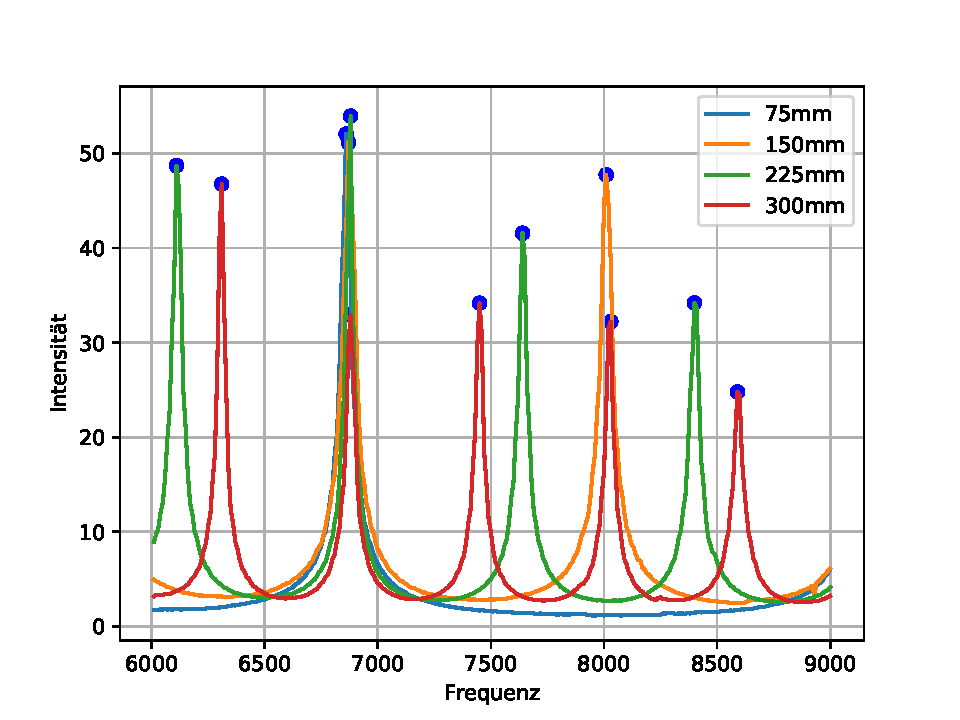
\includegraphics[width=\textwidth]{1234.pdf}
  \caption{Intensität der Schallwelle im Bereich von 6000 bis 9000 $\si{Hz}$ für die Rohrlängen $\SI{75}{mm}, \SI{150}{mm}, \SI{225}{mm}, \SI{300}{mm}$}
  \label{fig.1}
\end{figure}
In der Abbildung \ref{fig.2} sind die Messwerte für die Rohrlängen : $\SI{375}{mm}, \SI{450}{mm}, \SI{525}{mm}, \SI{600}{mm}$ abbgebildet.
\begin{figure}[h!]
  \centering
  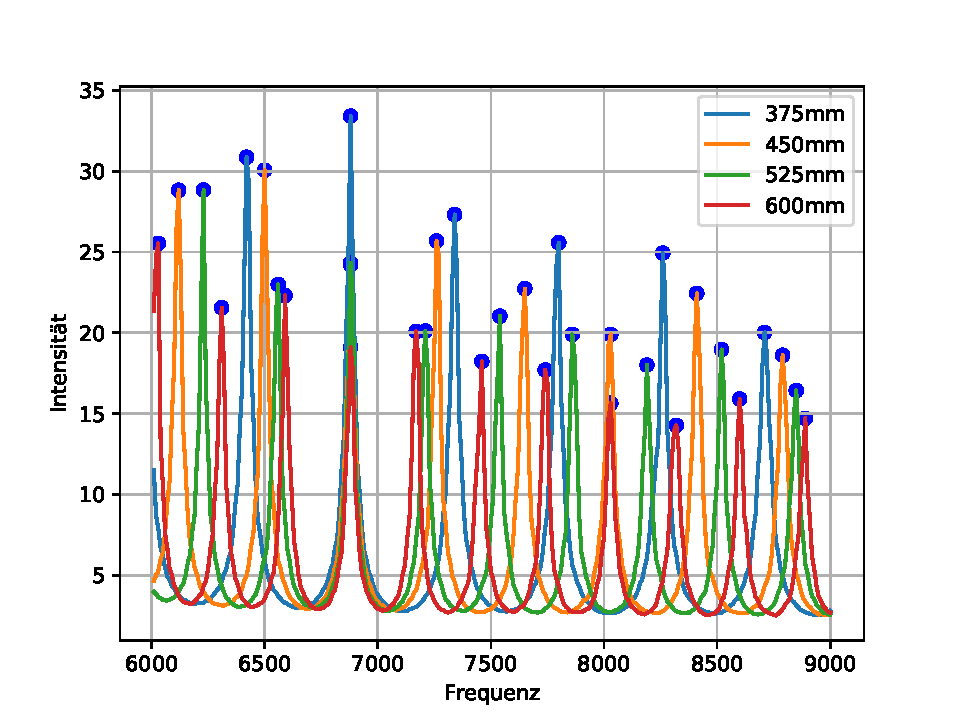
\includegraphics[width=\textwidth]{5678.pdf}
  \caption{Intensität der Schallwelle im Bereich von 6000 bis 9000 $\si{Hz}$ für die Rohrlängen $\SI{375}{mm}, \SI{450}{mm}, \SI{525}{mm}, \SI{600}{mm}$}
  \label{fig.2}
\end{figure}
Die Intensitätsmaxima sind mit einem blauen Punkt gekennzeichnet.
Auffällig ist, dass sich für alle Rohrlängen Intensitätsmaxima an der Stelle von $\SI{6880}{Hz}$ bilden. Das heißt, dass bei dieser Frequenz eine stehende Welle entsteht die eine Wellenlänge von $\lambda=\frac{1}{2n}d$ besitzt.
$d$ ist dabei die Länge des Rohres und n die Anzahl der Knotenpunkte.
Desweiteren ist auffällig, dass für eine Rohrlänge die Abstand zwichen zwei Maxima immer konstannt ist.

\subsection{Bestimmung der Lichtgeschwindigkeit}
In den Graphen \ref{fig.2} und \ref{fig.2} werden die Resonanzfrequenzen einer jeden Messreihe von 1 bis n nummeriert und anschließend gegen die Frequenz aufgetragen.
Die Resonazfrequenzabstände sind konstant für eine Messreihe, daher ergeben sich Geraden der Form: $y=ax+b$ welche an die Messwerte gefittet werden.
In der Abb. \ref{fig.linearfit} sind die Messwerte mit den Fitfunktionen abgebildet.
%Für die Fitparameter ergeben sich folgende Werte.
%\begin{align*}
%  a &= 286.54545455 \pm 0.37848474\\
%  b &= 5737.09090907 \pm 2.56700835
%\end{align*}
Mit Hilfe der Steigung $a$ kann die Schallgeschwindigkeit $c$ berechnet werden.
\begin{align*}
  c = a\cdot2d
\end{align*}
Für die Schallgeschwindigkeit ergeben sich so Werte von:
\begin{align*}
a &= 1140.0 && d = 2\cdot\SI{0.075}{m} && c=\SI{342.0}{\frac{m}{s}}\\
a &= 763.0  && d = 3\cdot\SI{0.075}{m} && c=\SI{343.3}{\frac{m}{s}}\\
a &= 571.0  && d = 4\cdot\SI{0.075}{m} && c=\SI{342.6}{\frac{m}{s}}\\
a &= 458.6  && d = 5\cdot\SI{0.075}{m} && c=\SI{343.9}{\frac{m}{s}}\\
a &= 381.9  && d = 6\cdot\SI{0.075}{m} && c=\SI{343.7}{\frac{m}{s}}\\
a &= 327.2  && d = 7\cdot\SI{0.075}{m} && c=\SI{343.5}{\frac{m}{s}}\\
a &= 286.5  && d = 8\cdot\SI{0.075}{m} && c=\SI{343.8}{\frac{m}{s}}\\
\end{align*}
Der Mittelwert ergibt:
\begin{align*}
  c=\SI{343.28\pm1.63}{\frac{m}{s}}.
\end{align*}
%###########Bild##########
%\begin{figure}[h!]
%  \centering
%  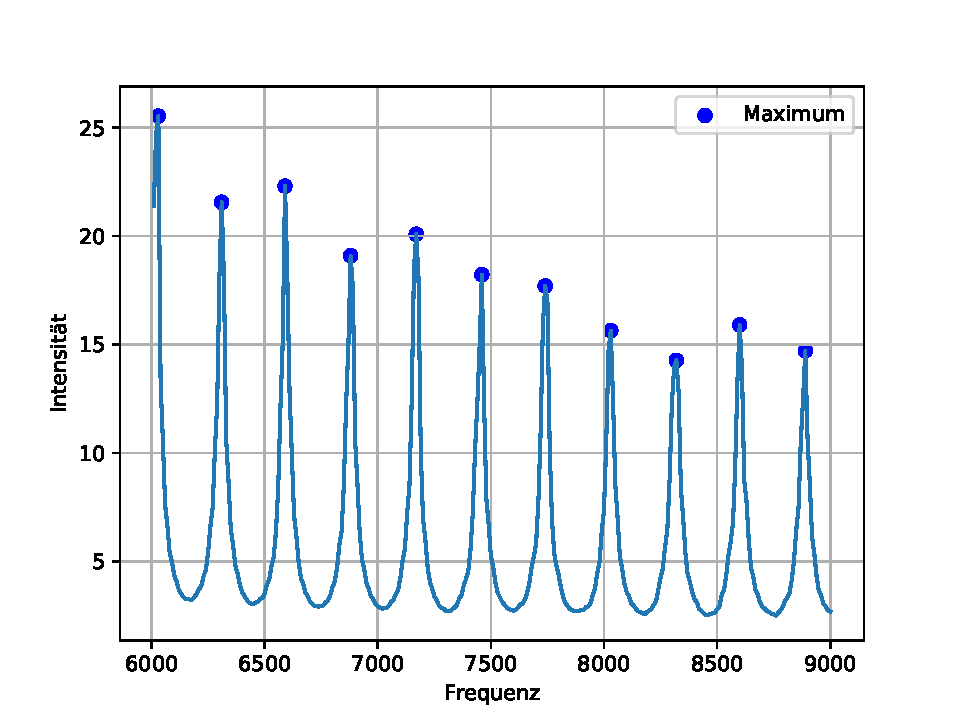
\includegraphics[width=\textwidth]{A1L8x75mmF6000-9000S10.pdf}
%  \caption{Messung eines $\SI{0.6}{m}$ Rohres für den Frequenzbereich von 6000 bis 9000 Hz}
%  \label{fig.frequenz/rohrlänge}
%\end{figure}
\begin{figure}[h!]
  \centering
  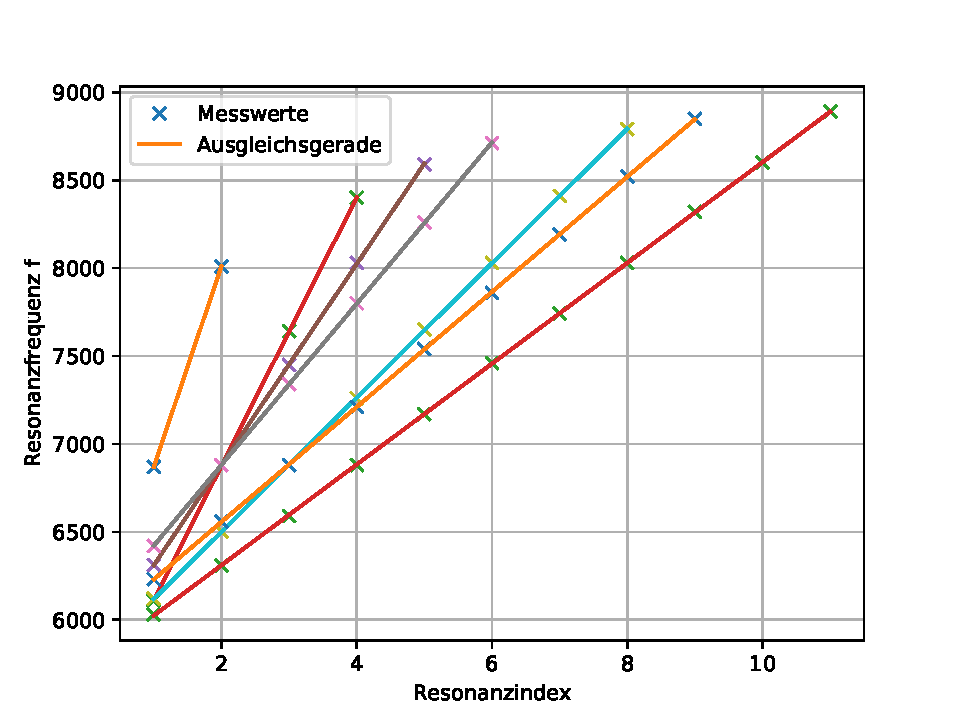
\includegraphics[width=\textwidth]{linearfit.pdf}
  \caption{Die Intensitätsmaxima werden nummeriert und die Nummer gegen die Frequenz aufgetragen.}
  \label{fig.linearfit}
\end{figure}
%#########
\FloatBarrier
Die Schallgeschwindigkeit kann auch mit Hilfe einer anderen Methode bestimmt werden.
dazu betrachten wir ein Rohr der Länge $\SI{75}{mm}$ für die Frequenzen von 6000 bis 9000 $\si{Hz}$.
Da die Rohrlänge $d$ ein vielfaches $n$ der halben Wellenlänge $\lambda$ ist gilt:
\begin{align*}
  \lambda = \frac{2d}{n}.
\end{align*}
Die Schallgeschwindigkeit ist gegeben durch:$c=f \cdot \lambda$.
Daraus ergibt sich :
\begin{align*}
  n&=1  c&=\SI{1032}{\frac{m}{s}}\\
  n&=2  c&=\SI{516}{\frac{m}{s}}
\end{align*}
\begin{align}
  n&=3  c&=\SI{344}{\frac{m}{s}}
  \label{eqn.schall}
\end{align}
\begin{align*}
  n&=4  c&=\SI{258}{\frac{m}{s}}.
\end{align*}
Die Freqenz ist dabei gegeben als $\SI{6880}{\frac{m}{s}}$.
Diese Freqenz ist die einzige Frequenz im Frequenzbereich welche bei allen Vielfachen der Rohrlänge von $\SI{75}{mm}$ vertreten ist,
zusehen ist dies in den Abb. \ref{fig.1} und \ref{fig.2}.
\textbf{\huge{Den Ergebnissen aus \ref{eqn.schall} ist zu entnehmen, dass die Wellenlänge bei $\frac{3}{2}\lambda$ liegt, da die dazugehörige Schallgeschwindigkeit von $\SI{344}{\frac{m}{s}}$ gut zum Literaturwert??? von $\SI{343.2}{\frac{m}{s}}$ passt.}}

\FloatBarrier
Desweiteren soll die Schallgeschwindigkeit mithilfe des Verhältnisses von Frequenzübergang zu Rohrlänge bestimmt werden.
Dieser Zusammenhang ist in Abb. \ref{fig.1/x} dargestellt.
An die Messwerte wird eine Funktion der Form $a\cdot\frac{1}{x}+b$ gefittet.
Für a und b ergegben sich die Werte:
\begin{align*}
  a&=1.68692913\cdot10^5\pm253.97695158\\
  b&=8.56657992\pm1.99530368\\
\end{align*}
%################Bild#####################
\begin{figure}[h!]
  \centering
  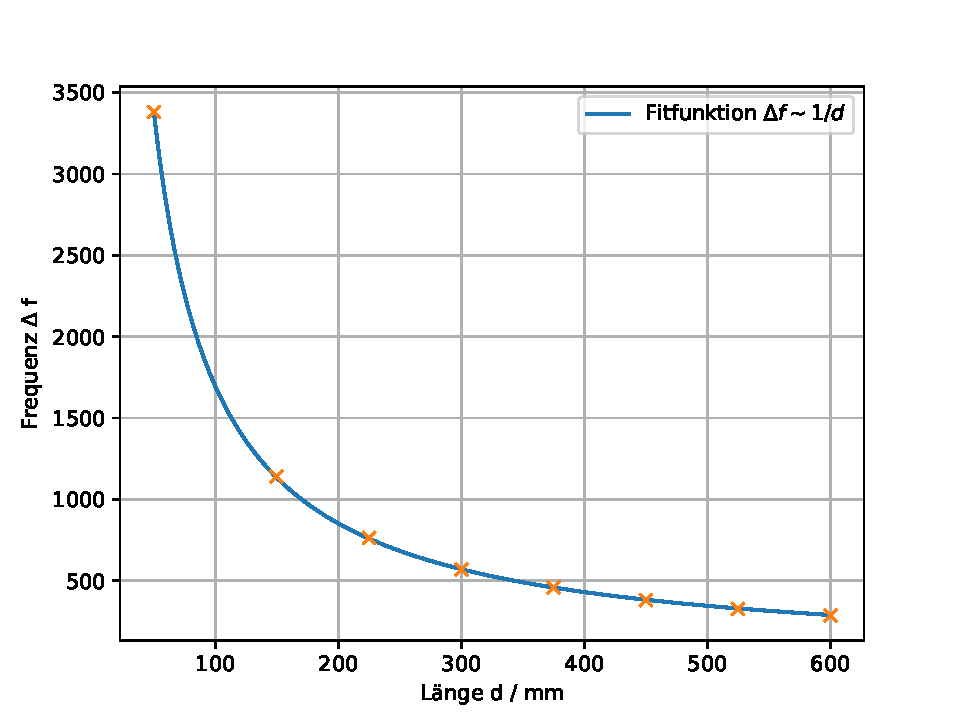
\includegraphics[width=\textwidth]{geschi.pdf}
  \caption{Der Abstand der Frequenzen wird gegen die Rohrlänge Aufgretragen.}
  \label{fig.1/x}
\end{figure}
\FloatBarrier

\subsection{Aufgabe 2: Dispersion}
In dieser Aufgabe wird $f(k)$ geplottet.
Aus der Messung mit einer Rohrlänge von $12\cdot\SI{50}{mm}$ und einem Frequenzbereich von $400-12000\si{Hz}$ werden die Maximalstellen mit Hilfe einer Peak-Piking ermittelt.
Die Maximalstellen werden durchnummerriert und die darugehörige Freqenz in $f(k)$ ungerechnen.
\begin{align}
  k= \frac{n \pi}{L}
\end{align}
$L$ ist dabei die gesammte Rohrlänge.

In der Abbildung \ref{fig.Aufgabe2} ist $k$ gegen $f(k)$ aufgetragen. Dargestellt ist zu einen die Dispersionsrelation von Schallwellen und zum anderen die Diespersionsrelation eines quantenmechanischen Teilchens im Potenzialtopf nach der Funktion \ref{eqn:dispersionqm}
Es ist zu erkennen, dass die Dispersion von Schalwellen linear verläuft wohingegen die Dispersion eines quantenmechanischen Teilchens im Potenzialtopf quadratisch ist.
Das Analogon zwischen den belden Dispersionsrelationen ist daher nicht sehr zutreffend.
\begin{figure}[h!]
  \centering
  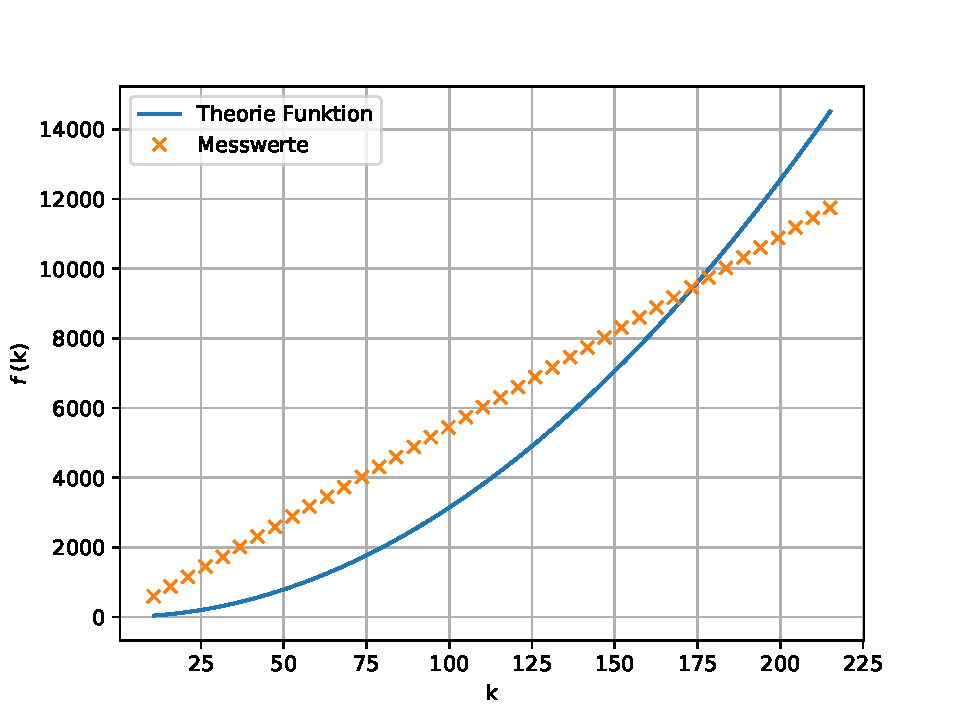
\includegraphics[width=\textwidth]{f(k).pdf}
  \caption{Dispersionsrelation für Schalwellen X und die Theorikurve eines quantenmechanischen Teilchens im Potenzialtopf}
  \label{fig.Aufgabe2}
\end{figure}
\FloatBarrier

\subsection{Aufgabe 3: Bandstruckturen}
In dieser Aufgabe werden die Bandlücken in reation zu der Blendengröße gesetzt.
Anhand der Abbildung \ref{fig.Aufgabe3} wird deutlich, dass die Bandlücken mit zunehmender Blendengröße kleiner werden.
Die Bandlücken wirden bestimmt indem man die Differenz vom Anfang und Ende der Bandlücke betrachtet.
\begin{figure}[h!]
  \centering
  \includegraphics[width=\textwidth]{Bandlücken3.pdf}
  \caption{Größe der Bandlücken aufgetragen gegen die Blendengröße}
  \label{fig.Aufgabe3}
\end{figure}
\FloatBarrier

\subsection{Aufgabe 4: Bandstruckturen}
Diese Aufgabe ist sehr ähnlich zur Aufgabe 3. Hier wird die Bandlücke jedoch im Verhältniss zur Rohrlänge betrachtet.
Dementsprechend ist in der Abbildung \ref{fig.Aufgabe4} die Badlücken gegen die Rohrlängen aufgetragen.
Die Rohrlänge wird zwichen 8, 10 und 12 mal $\SI{50}{mm}$ variiert.
Die Messung ist nicht sehr aussagekräftig.
Lediglich ist zu erkennen, dass die Bandlücken relativ unabhängig von der Rohrlänge sind.
\begin{figure}[h!]
  \centering
  \includegraphics[width=\textwidth]{Bandlücken.pdf}
  \caption{Größe der Bandlücken aufgetragen gegen die Rohrlänge}
  \label{fig.Aufgabe4}
\end{figure}
\FloatBarrier

\subsection{Aufgabe 5}
In Dieser Aufgabe wird die Bandlücke ebenfals ins Verhältniss mit der Rohrlänge genommen. Dabei wir zwichen 8 mal $\SI{75}{mm}$ und 8 mal $\SI{50}{mm}$ gewechselt.
Es werden dementsprächend unterschiedlich große Einheitszellen betrachtet.
In den Abbildungen \ref{fig.Aufgabe5} und \ref{fig.Aufgabe575} sind die Maxima gegen k geplottet. Anhand der hinterlegten Bandlücken wird deutlich, dass die Bandlücken für größere Rohrabschnitte kleiner werden.
In der Abbildung \ref{fig.Aufgabe5a} wird ebenfals deutlich, dass die größe der Bandlücke fällt mit größeren Einheitszellen.
%\FloatBarrier

\begin{figure}
 \centering
 \begin{subfigure}{0.48\textwidth}
  \centering
  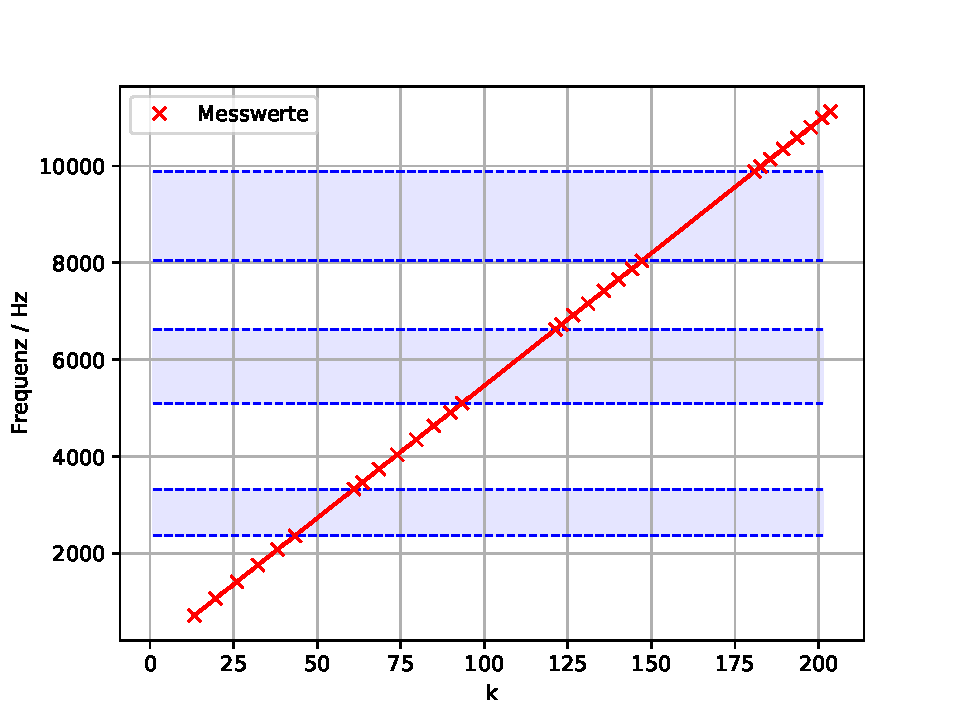
\includegraphics[width=1\textwidth]{bla.pdf}
  \caption{8 mal \SI{50}{mm}}
  \label{fig.Aufgabe5}
 \end{subfigure}
 \begin{subfigure}{0.48\textwidth}
  \centering
  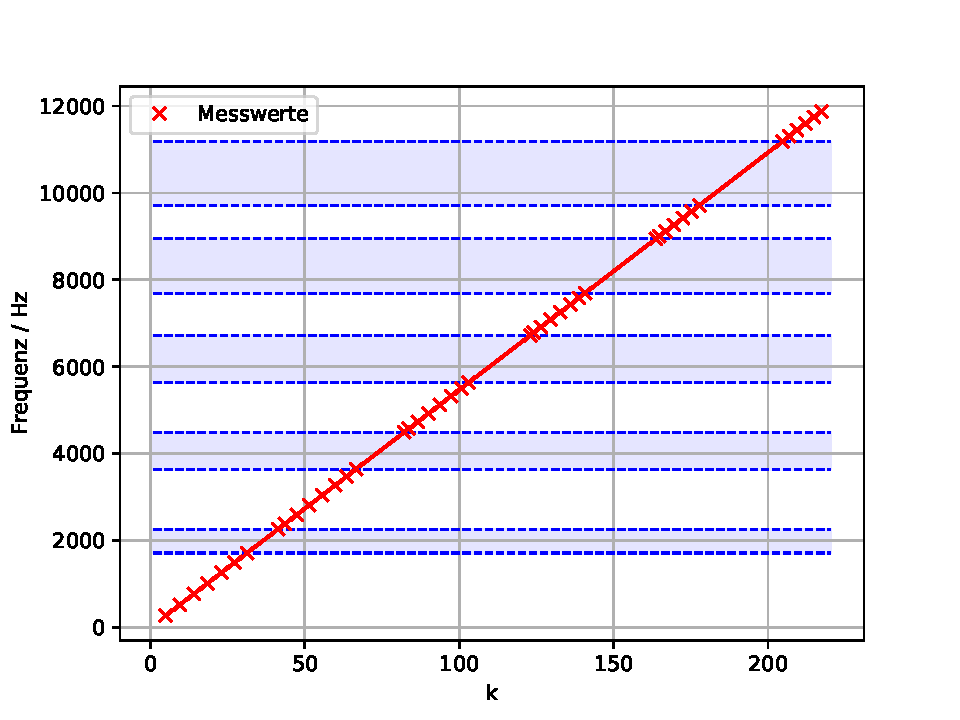
\includegraphics[width=1\textwidth]{bla75.pdf}
  \caption{8 mal \SI{75}{mm}}
  \label{fig.Aufgabe575}
 \end{subfigure}
 \caption{Bandlücken für unterschiedliche Rohrlängen}
 %\label{fig:500-6-7}
\end{figure}

\begin{figure}[h!]
  \centering
  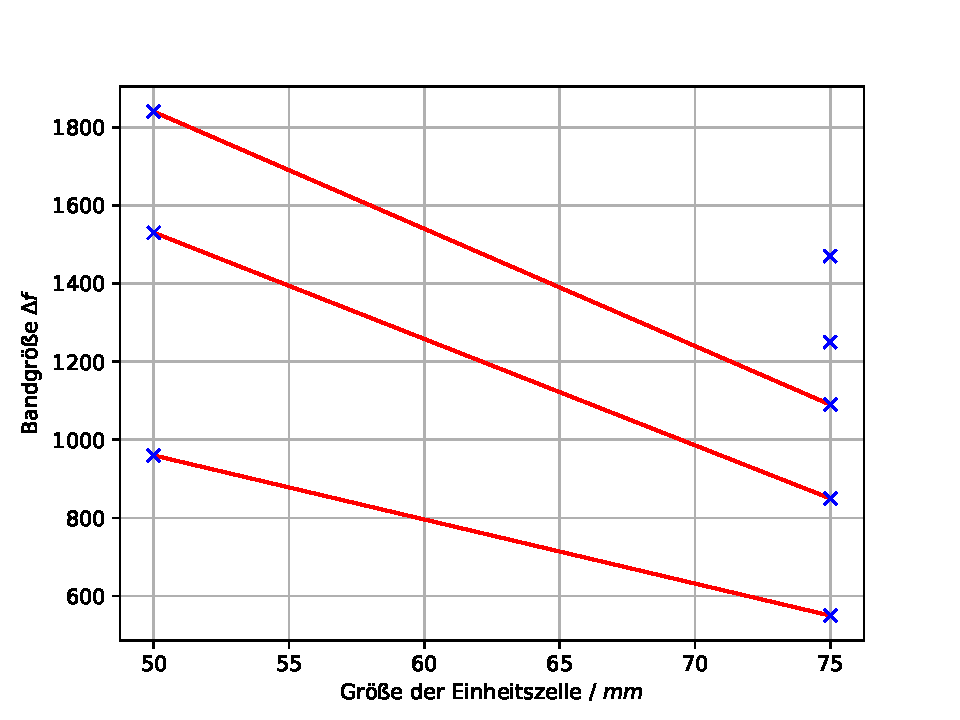
\includegraphics[width=\textwidth]{newtest.pdf}
  \caption{Größe der Bandlücken aufgetragen gegen die größe der Einheitszelle}
  \label{fig.Aufgabe5a}
\end{figure}
\FloatBarrier

\subsection{Aufgabe 6 und 7}
In dieser Aufgabe werden wieder die Maxima gegen k geplottet. Es entsteht wieder wie erwartet eine Gerade wie in Abbildung \ref{fig.Aufgabe6} und \ref{fig.Aufgabe7} zusehen.
Anhand der Abbildungen ist zu sagen, dass sich die beiden Messungen nicht viel unterscheiden.

\begin{figure}
 \centering
 \begin{subfigure}{0.48\textwidth}
  \centering
  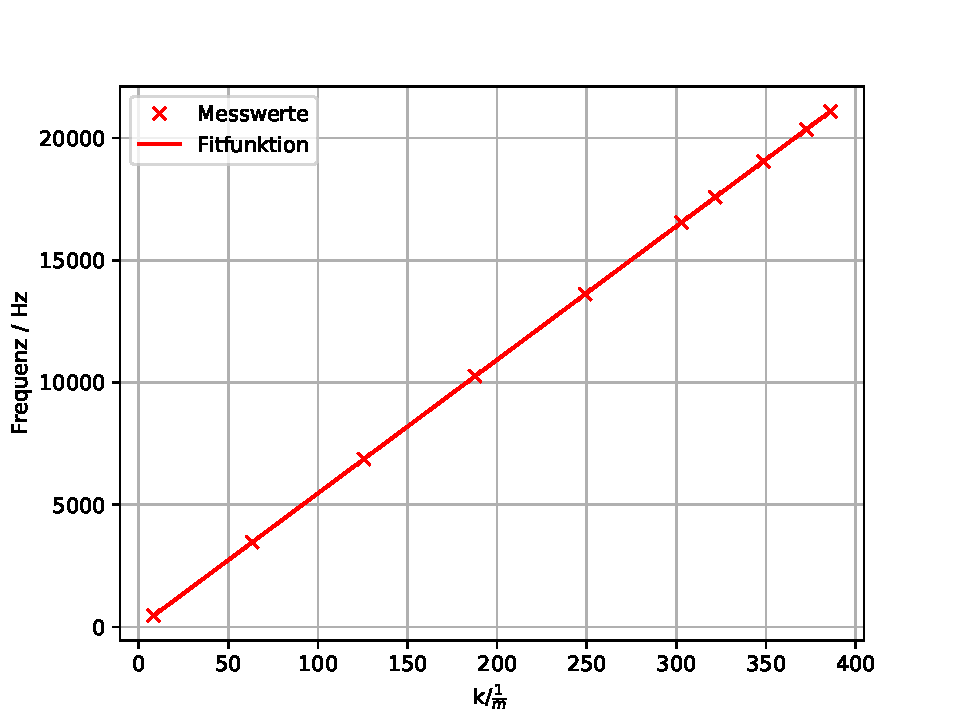
\includegraphics[width=1\textwidth]{A6.pdf}
  \caption{1 mal \SI{50}{mm}}
  \label{fig.Aufgabe6}
 \end{subfigure}
 \begin{subfigure}{0.48\textwidth}
  \centering
  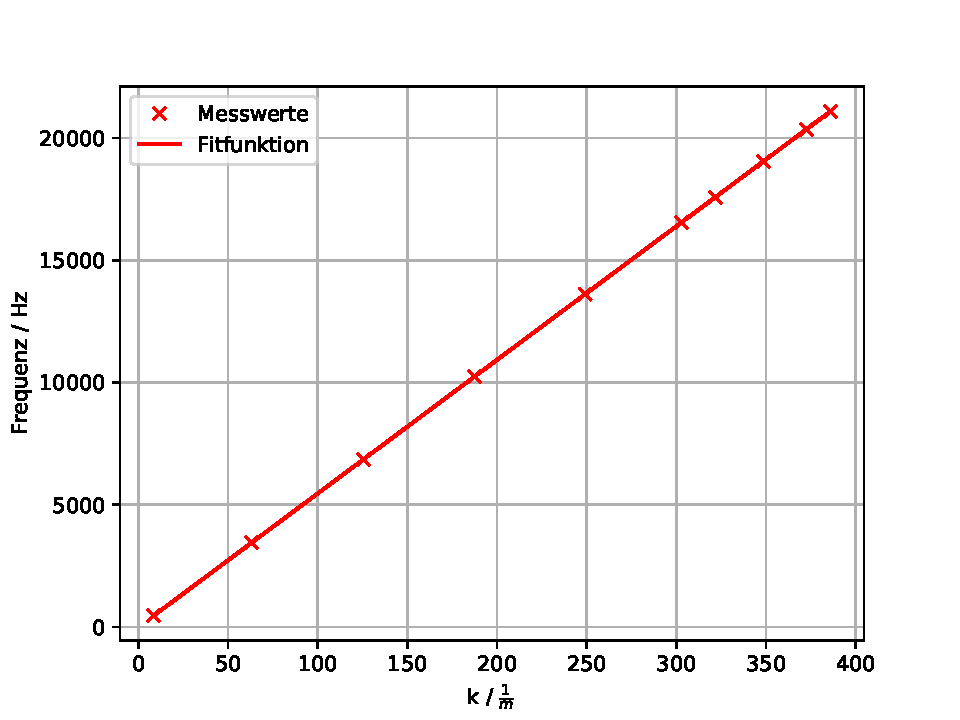
\includegraphics[width=1\textwidth]{A7.pdf}
  \caption{1 mal \SI{75}{mm}}
  \label{fig.Aufgabe7}
 \end{subfigure}
 \caption{Maxima gegen k}
 %\label{fig:500-6-7}
\end{figure}

\subsection{Aufgabe 8}
Es werden für 2 mal $\SI{50}{mm}$ Rohrlänge unterschiedliche Blendendurchmesser untersucht. Der Blendendurchmesser soll die Stärke von Bindungen zwischen Atomen symbolisieren.
Für die unterschiedlichen Blendendurchmesser entstehen unterschiedlich breite Bandlücken.
In der Abbidung $\ref{fig.Aufgabe8}$ ist der zusammenhang zwischen Blendendurchmesser und Bandlücke dargestellt.
Es wird deutlich dass bei größeren Blendendurchmessern die Bandlücken kleiner werden.
\begin{figure}[h!]
  \centering
  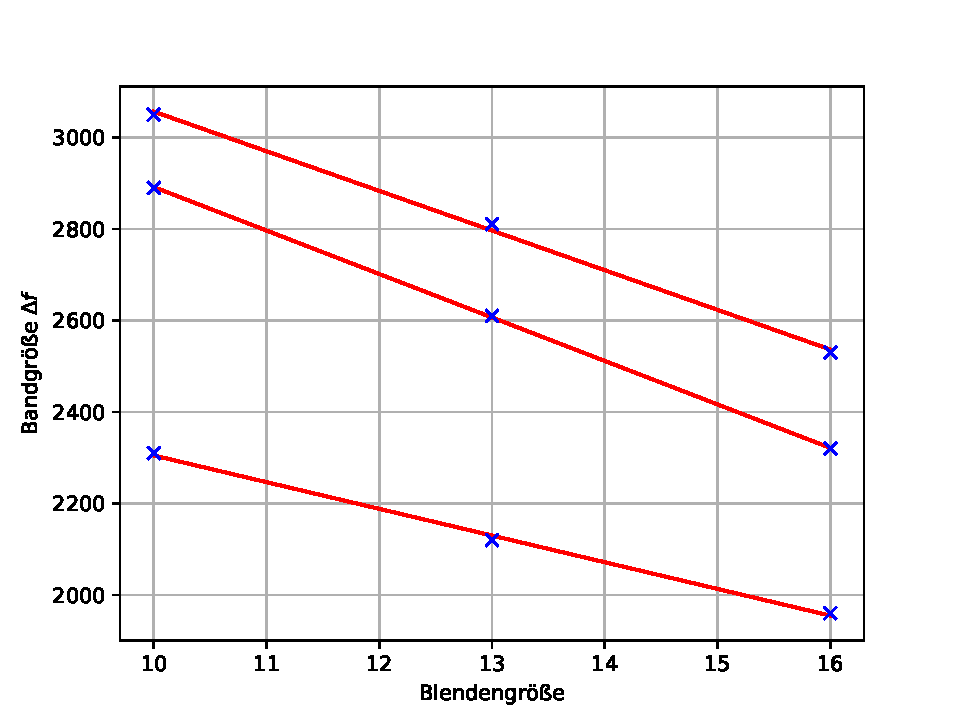
\includegraphics[width=\textwidth]{A8.pdf}
  \caption{Bandlücke in Abhängigkeit von dem Blendendurchmesser}
  \label{fig.Aufgabe8}
\end{figure}
\FloatBarrier
